\documentclass[12pt]{report}
\usepackage{fontspec}
  \setmainfont{Proxima Nova}
\usepackage[a4paper, portrait, margin=1in]{geometry}
\title{\textbf{Matrix Multiplier Verilog HDL}}
\author{Vishwas Rajashekar \\
Department of Computer Science and Engineering \\
PES University\\
Bangalore}
\date{}
\usepackage{graphicx}
\usepackage{amsmath}
\begin{document}

\maketitle

\section{Abstract}
Matrix operations form the foundation for Linear Algebra and consequently are the basis for image manipulation. In order to improve the wall clock time of image processing applications and to facilitate image alteration on lower end machines, it is important to accelerate matrix and floating point operations.
GPUs currently employ high levels of instruction level parallelism and parallel computing in order to provide these features.
This project aims to demonstrate how matrix multiplication and addition can be performed by hardware by displaying an HDL representation and simulation of combinational logic.

\section{Concept}
This project aims to employ the basic concept of how matrix multiplication works in order to design combinational logic to perform the same.
\begin{figure}[htp]
\centering
\includegraphics[scale=1.00]{/home/darkaether0x1/Downloads/Papers/2-bit-multiplication-new.png}
\caption{Parallel Binary Multiplication \cite{binmult}}
\label{}
\end{figure}
\begin{figure}[htp]
\centering
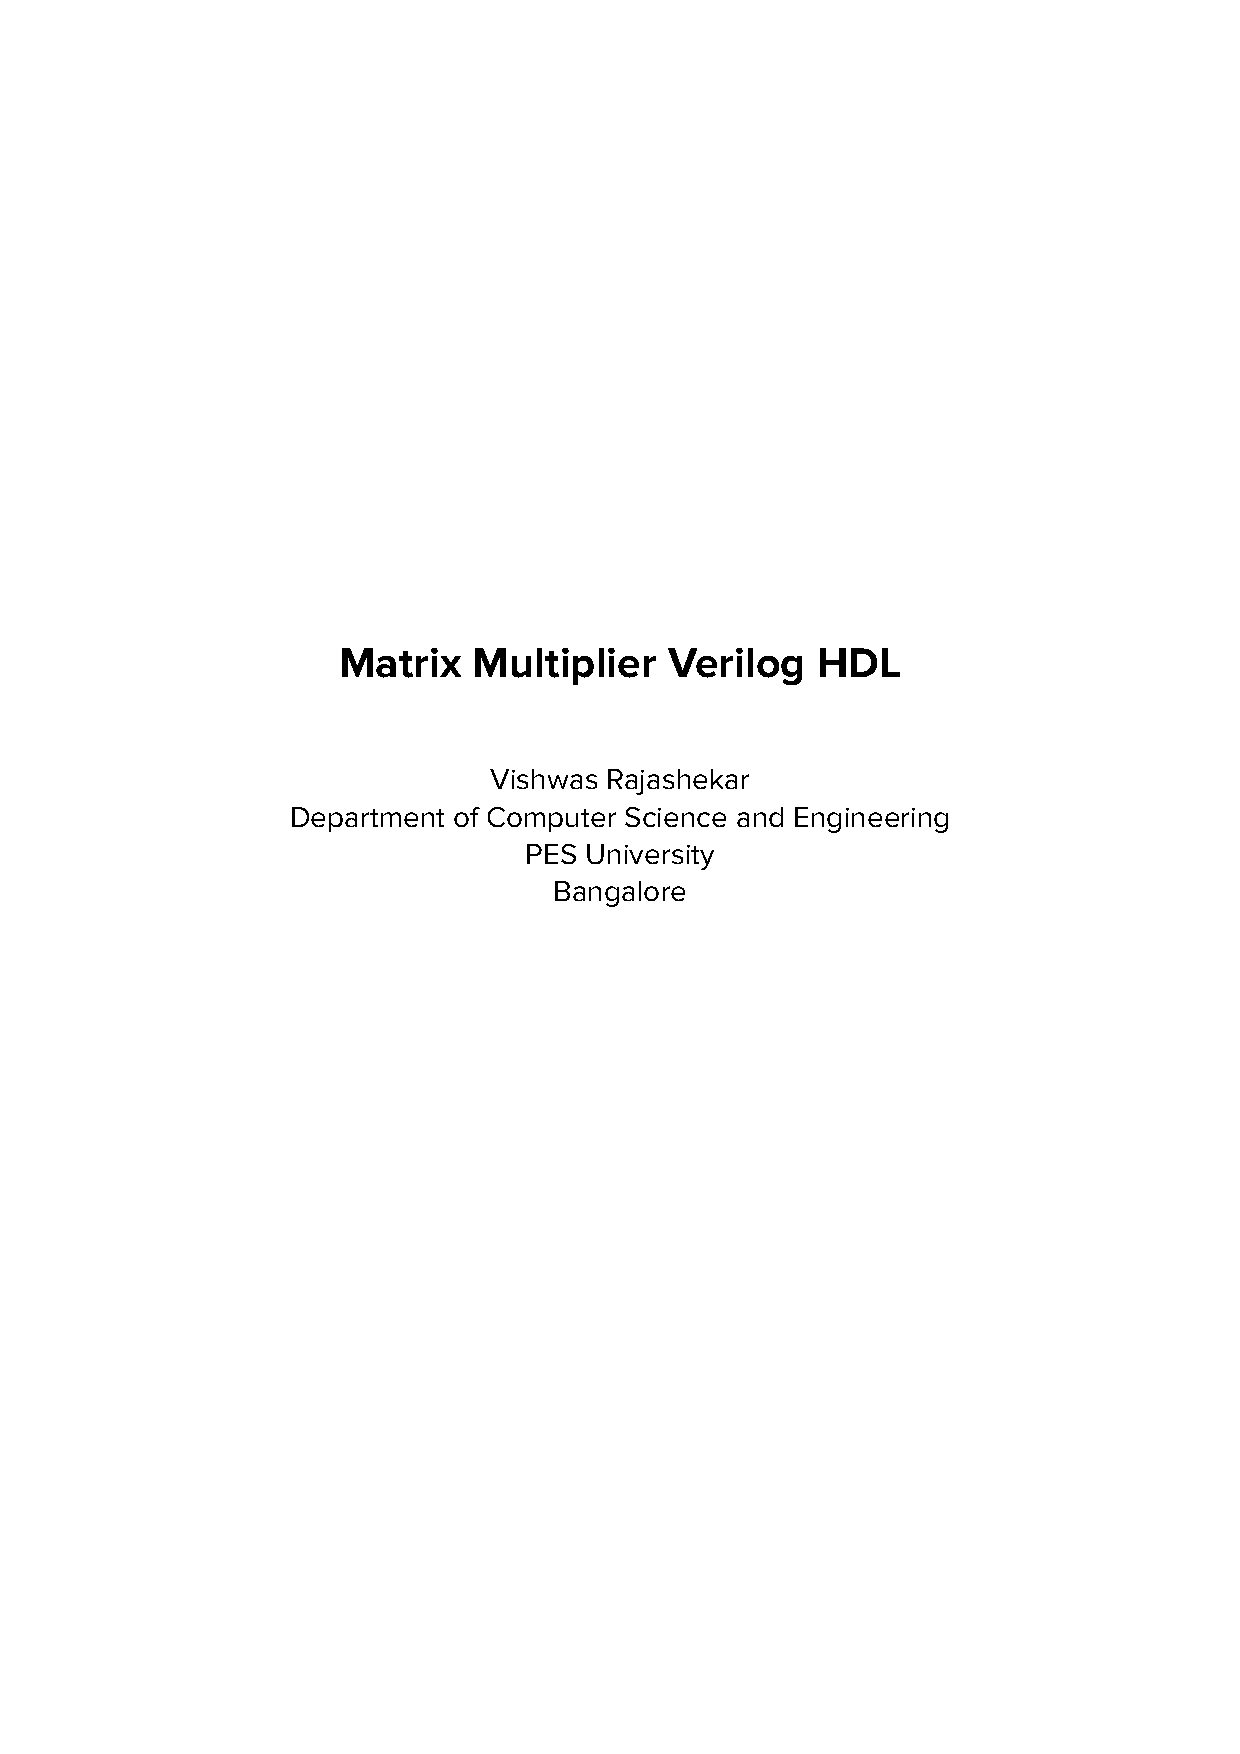
\includegraphics[scale=1.00]{/home/darkaether0x1/Downloads/Papers/mat_mult.png}
\caption{Matrix Multiplication}
\label{}
\end{figure}
\section{Design}
\newpage
\vfill
\begin{figure}[htp]
\centering
\includegraphics[scale=0.85]{/home/darkaether0x1/Downloads/Papers/4bitmult.png}
\caption{2x2 matrix multiplier}
\label{}
\end{figure}

Design of a 4 x 4 matrix multiplier using the above Divide and Conquer concept:
$$
\begin{bmatrix} 
a & b & c & d\\
e & f & g & h\\
i & j & k & l\\
m & n & o & p\\
\end{bmatrix}
\times
\begin{bmatrix} 
a1 & b1 & c1 & d1\\
e1 & f1 & g1 & h1\\
i1 & j1 & k1 & l1\\
m1 & n1 & o1 & p1\\
\end{bmatrix}
=
\begin{bmatrix} 
q & r & s & t\\
u & v & w & x\\
y & z & a2 & b2\\
c2 & d2 & e2 & f2\\
\end{bmatrix}
$$
\vfill
\clearpage
\section{Simulation}
$$
\begin{bmatrix} 
1 & 2 \\
3 & 4 
\end{bmatrix}
\times
\begin{bmatrix} 
5 & 6 \\
7 & 8 
\end{bmatrix}
=
\begin{bmatrix} 
19 & 22 \\
43 & 50 
\end{bmatrix}
$$
$$
\begin{bmatrix} 
5 & 5 \\
5 & 5 
\end{bmatrix}
\times
\begin{bmatrix} 
5 & 5 \\
5 & 5 
\end{bmatrix}
=
\begin{bmatrix} 
50 & 50 \\
50 & 50
\end{bmatrix}
$$
$$
\begin{bmatrix} 
1 & 2 \\
5 & 4 
\end{bmatrix}
\times
\begin{bmatrix} 
5 & 5 \\
7 & 8 
\end{bmatrix}
=
\begin{bmatrix} 
19 & 21 \\
53 & 57
\end{bmatrix}
$$
$$
\begin{bmatrix} 
4 & 3 \\
2 & 1 
\end{bmatrix}
\times
\begin{bmatrix} 
8 & 7 \\
6 & 5 
\end{bmatrix}
=
\begin{bmatrix} 
50 & 43 \\
22 & 19
\end{bmatrix}
$$
$$
\begin{bmatrix} 
0 & 1 \\
2 & 0 
\end{bmatrix}
\times
\begin{bmatrix} 
0 & 1 \\
2 & 0 
\end{bmatrix}
=
\begin{bmatrix} 
2 & 0 \\
0 & 2
\end{bmatrix}
$$

\begin{figure}[htp]
\centering
\includegraphics[scale=1.00]{/home/darkaether0x1/Downloads/Papers/sim.png}
\caption{Simulation of 2x2 Matrix Multiplier}
\label{}
\end{figure}
\vfill
\clearpage
\section{Conclusion}
Combinational Logic can be implemented in hardware in order to speed up matrix multiplication by exploiting the parallelism that a hardware implementation offers, as opposed to a software approach.
\begin{thebibliography}{999}

\bibitem{binmult}
  ElectronicsHub, Binary Multiplication
  \begin{verbatim}https://www.electronicshub.org/binary-multiplication/\end{verbatim}
\bibitem{matmult}
  GeeksforGeeks, Matrix Multiplication
  \begin{verbatim}https://www.geeksforgeeks.org/strassens-matrix-multiplication/\end{verbatim}
\end{thebibliography}
\end{document}
